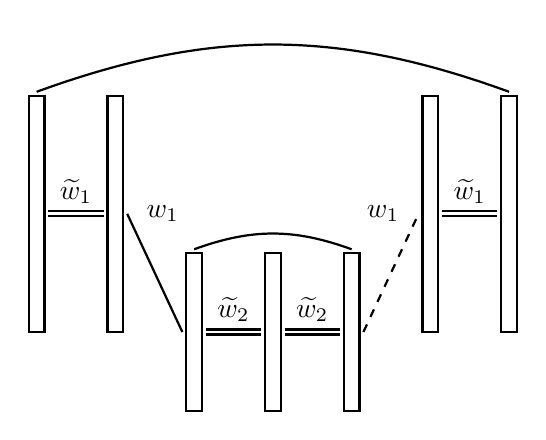
\begin{tikzpicture}[x=1cm,y=1cm]
  \tikzset{
    smooth/.style={thick, double, double distance=1pt},
    stride/.style={thick},
    upsample/.style={thick, dashed},
    skip/.style={thick}
  }

  % Upper-left encoder pair
  \draw[black, thick] (0,-1.5) rectangle (0.2, 1.5);
  \coordinate (ULtop) at (0.1, 1.55);
  \draw[smooth] (0.25,0) -- (0.95,0) node[above, midway] {$\widetilde{w}_1$};
  \draw[black, thick] (1.0,-1.5) rectangle (1.2, 1.5);

  % Downsample to lower level
  \draw[stride] (1.25,0) -- (1.95,-1.5);
  \node at (1.7, 0) {$w_{1}$};

  % Bottom (coarser) path: three blocks with two smooth convolutions
  \draw[black, thick] (2.0,-2.5) rectangle (2.2, -0.5);
  \coordinate (L1top) at (2.1, -0.45);

  \draw[smooth] (2.25,-1.5) -- (2.95,-1.5) node[above, midway] {$\widetilde{w}_2$};
  \draw[black, thick] (3.0,-2.5) rectangle (3.2, -0.5);

  \draw[smooth] (3.25,-1.5) -- (3.95,-1.5) node[above, midway] {$\widetilde{w}_2$};
  \draw[black, thick] (4.0,-2.5) rectangle (4.2, -0.5);
  \coordinate (L3top) at (4.1, -0.45);

  % Bottom skip connection
  \draw[skip] (L1top) to[out=20,in=160] (L3top);

  % Transposed operation back to upper level
  \draw[upsample] (4.25,-1.5) -- (4.95,0);
  \node at (4.5, 0) {$w_{1}$};

  % Upper-right decoder pair
  \draw[black, thick] (5.0,-1.5) rectangle (5.2, 1.5);
  \draw[smooth] (5.25,0) -- (5.95,0) node[above, midway] {$\widetilde{w}_1$};
  \draw[black, thick] (6.0,-1.5) rectangle (6.2, 1.5);
  \coordinate (URtop) at (6.1, 1.55);

  % Top-level skip connection
  \draw[skip] (ULtop) to[out=20,in=160] (URtop);
\end{tikzpicture}